\chapter{Object Reconstruction}
\label{sec:object_reconstruction}

\section{Tracks and vertices}

The reconstructed vertex with the largest value of summed physics-object $\pT^{2}$ is taken to be the primary pp interaction vertex. 
The physics objects for this purpose are the jets, clustered using the jet finding algorithm~\cite{Cacciari:2008gp,Cacciari:2011ma}, as described below, with the tracks assigned to the vertex as inputs, and the
associated missing transverse momentum, taken as the negative vector sum of the $\pT$ of those jets.
Any other collision vertices in the event are associated with additional soft inelastic pp collisions called \emph{pileup}.

\section{Particle flow}

The particle-flow (PF) algorithm reconstructs the products of the LHC pp collisions and is described in full in Ref.\cite{PF_CMS}.  
It utilises all the information available from the tracker, ECAL, HCAL and muon detectors combined to produce a list of particle candidates. 
These candidates are either a photon, electron, muon or a neutral or charged hadrons. It begins with defining an event as the data taken per bunch crossing. 
The PF algorithm then reconstructs the tracks of the particle candidates in order to find the collision vertices. 
The primary collision vertex is taken to be the one with the largest value of \(p_T^{2}\) summed over all physics objects originated from that vertex. 
Physics objects are not only defined to include particle candidate tracks, but also missing tracks represented by the negative vectorial sum of all particle candidate tracks. Other pp collisions vertices are referred to as pileup. \\

In reconstructing electron and muons, the energy deposits in the ECAL and the track hits in the muon chamber respectively, working alongside the tracker, provide the basis of electron and muon identification. However, additional requirements are used to drop misidentification rates by ensuring that the electron or muon is isolated from any hadronic activity in the detector, as leptons do not carry colour charge. This is done by defining a relative isolation variable \(I_{rel}^{e(\mu)}\) in the following way

\begin{equation}
    I_{rel}^{e\mu} = \frac{\sum p_{T,i} + \sum E_{T,i}}{p_T^{e\mu}}.
\end{equation}

The sums are over all particles included in a cone of radius \(\Delta R = \sqrt{(\Delta \eta)^2 + (\Delta \phi)^2}\) excluding the electron or muon itself. \(\Delta \eta\) and \(\Delta \phi\) are the angular distance in \(\eta\) and \(\phi\) around the electron or muon direction from the primary vertex. To remove problems with pileup, only charged particles originating from the primary vertex are included. To remove neutral particles from pileup in the cone, the \(p_T\) for neutral particles is estimated by subtracting half of the sum of the \(p_T\) of charged particle in the cone, due to the approximate ratio of charged to neutral hadron production. The cone size selected for electrons is \(\Delta R<0.3\) and the isolation variable is \(I_{\text{rel}}^{e(\mu)} < 0.1\). For muons is cone size is \(\Delta R<0.4\) and the isolation variable is \(I_{\text{rel}}^{e(\mu)} < 0.15\). \\

Jets originating from the hadronisation of b quarks, are identified using the combined secondary vertex b-tagging algorithm. This discriminates between jets originating from b quarks from other jets, utilising track impact parameters and secondary vertex related variables \cite{CMS_btag}. This plays a key part in the analysis, as b-tagging is used for categorisation purposes described in Section \ref{sec:cat_and_sig}. The missing transverse momentum, \(\vec{p}_T^{\hspace{1ex}\text{miss}}\), is also used in categorisation of events and is calculated as the negative vector sum of all PF reconstructed transverse momenta.

\section{Muons}

Muons are required to be reconstructed as muon by the particle flow reconstruction. They additionally must pass \textit{Medium muon} requirements~\cite{cmsMediumMuon}, 
as recommended by the Muon POG. These requirements are:
\begin{itemize}
\item The muon is reconstructed by the \textit{tracker} or \textit{global} muon reconstruction algorithm.
\item The impact parameters $d_{xy}$ and $d_{z}$ between the muon track ('best track') 
and the primary vertex are restricted as $d_{xy}<0.045$~cm and $d_{z}<0.2$~cm to ensure the muon is associated with the primary vertex
\item At least 80\% of the tracker hits have to be valid
\end{itemize}
In addition, either of the following two sets of criteria must be satisfied:
\begin{itemize}
\item The muon is reconstructed by the \textit{global} muon reconstruction algorithm.
\item The $\chi^2$/ndof of the global track fit is smaller than 3
\item The $\chi^2$ of the tracker-standalone position match is smaller than 12
\item The $\chi^2$ of the track kink finder is less than 20
\item The muon segment compatibility is $>$ 0.303
\end{itemize}
\textit{or}:
\begin{itemize}
\item The muon segment compatibility is $>$ 0.451 
\end{itemize}

\textbf{Isolation}~\\
To reduce the contamination from muons originating from heavy-flavoured quark decays in jets or decays in flight, selected muons are required to be isolated. The isolation is based on photon and neutral/charged hadron particle flow candidates within a cone size of $\Delta R<0.4$ of the selected muon. A relative combined isolation variable is defined as:

\begin{equation}
\label{eqn:reliso}
I_{rel}^{\mu} = \frac{\Sigma P_{T}(\text{charged}) + \mathrm{max}(\Sigma E_{T}(\text{neutral}) + \Sigma E_{\text{T}}(\text{photon}) - \Delta\beta \Sigma E_{\text{T}}(\text{PU}),0)}{P_{\text{T}}^{\mu}},
\end{equation}

where $P_{T}(\text{charged})$ corresponds to the $P_{T}$ of all charged hadronic candidates from primary vertex, $E_{T}(\text{photon, neutral})$ 
to the transverse energy of all photon and neutral hadron candidates, and $\Delta \beta$ is the energy estimate of neutral particles due to pileup, which is taken to be 0.5.
Furthermore $E_{\text{T}}(\text{PU})$ corresponds to the transverse momentum of all charged hadronic candidates from pileup.
The muon isolation used is $I_{rel}<0.15$.

\section{Electrons}

In addition, electrons are required to pass an identification variable based on a Boosted Decision Tree (BDT) 
discriminator which uses track quality, shower shapes and kinematic quantities as input.
The following variables are used as input to the BDT:  ~\cite{cmsElectron}
\begin{itemize}
\item Cluster shape variables $\sigma_{i\eta,i\eta}$ and $\sigma_{i\phi,i\phi}$, with $i\eta$ and $i\phi$ the integer
label of the $\eta$ and $\phi$ calorimeter cell. The circularity =  $1 -\frac{E1\times5}{E5\times5}$, with
$E1\times5$ and $E5\times5$ the energies in a $1\times5$ and a $5\times5$ grid around the super cluster seed,
respectively. Shape variable R9 = $\frac{E3\times3}{E_{SC}}$, with $E3\times3$ the energy in a $3\times3$ grid
of cells around the super cluster seed and $E_{SC}$ the raw energy of the super cluster.
\item The number of valid hits in the track fit, the $\chi^2$ of the track fit and the $\chi^2$ of the GSFTrack fit
\item The number of GSFtrack hits, the number of expected missing inner hits and the result of the conversion vertex fit
\item The distance $\Delta \eta$ and $\Delta \phi$ between the reconstructed super cluster and the associated track at the position of the primary vertex, and the distance in $\eta$ between the super cluster and the track at the calorimeter surface.
\item H/E, the ratio of the hadronic energy over the electromagnetic energy in the super cluster and E/P, the ratio of the super cluster energy over the momentum of the track associated with the electron 
\item The ratio of the energy of the electron cluster and the momentum of the associated track, evaluated at the electron cluster,
 and $1/E_e - 1/P_e$, with $E_e$ the energy of the electron candidate and $P_e$ its momentum.
\end{itemize}
The BDT was trained on a $Z/\gamma^{*}$ Monte Carlo sample generated with
\texttt{MadGraph 5}, in 3 $\eta$ bins for electrons with $p_{\text{T}}>10$ GeV.
This analysis uses the version of the ID BDT without the isolation included in
the training, instead using an additional cut on the electron isolation. This
was shown to give similar performance to the version of the ID including the
isolation and makes defining side-band regions used for estimation of
backgrounds simpler.

The electron are additionally required to pass the 90\% efficiency working point. Finally electrons are also subject to the same impact parameter requirements as the
muons: the impact parameters $d_{xy}$ and $d_{z}$ between the electron track 
and the primary vertex are restricted as $d_{xy}<0.045$~cm and $d_{z}<0.2$~cm to
ensure the electron is associated with the primary vertex.

The isolation used is based on photon and neutral/charged hadron particle flow
candidates within a cone size of $\Delta R<0.3$ of the selected electron but
used a different method to estimate the neutral particles due to pileup, namely
the rho--effective-area method. The pileup in this method is estimated as
$PU=\rho\cdot\text{EA}$, where $\rho$ is the event-specific average pile-up
energy density per unit area in the $\phi$-$\eta$ plane and the EA is the
effective area specific to the given type of isolation. The rho--effective-area
subtracted relative combined isolation variable is defined as:
\begin{equation}
\label{eqn:electron_reliso_rho} 
I_{\text{rel}}^{e} = \frac{\Sigma
    P_{T}(\text{charged}) + \mathrm{max}(\Sigma E_{T}(\text{neutral}) + \Sigma
E_{T}(\text{photon}) - \rho\cdot\text{EA},0)}{P_{T}^{e}}, \end{equation} where
the $\text{EA}$ is measured in bins of $\eta$ as listed in Table
\ref{tab:EleEA}. The electron isolation used is $I_{rel}<0.15$. 

\begin{table}[htb]
\begin{center}
{\footnotesize
\begin{tabular}{|c|c|}
\hline
$\eta$ range & EA \\
\hline
0.0$\leq\eta<$1.0   &  0.1440 \\
1.0$\leq\eta<$1.479 &  0.1562 \\
1.479$\leq\eta<$2.0 &  0.1032 \\
2.0$\leq\eta<$2.2   &  0.0859 \\
2.2$\leq\eta<$2.3   &  0.1116 \\
2.3$\leq\eta<$2.4   &  0.1321 \\
2.4$\leq\eta<$5.0   &  0.1654 \\
\hline
\end{tabular}
} % end footnotesize
\end{center}
\caption{
 Electron effective areas used for the $\rho$-corrected isolation computation.
}
\label{tab:EleEA}
\end{table}

\section{Jets}

Jets are clustered from all particle flow 
candidates using the anti $k_{\text{T}}$ algorithm~\cite{Cacciari:2011ma} with a cone size parameter R=0.4. To reduce the contribution of jets that originate from 
pile--up vertices, charged hadrons that are not associated with the hard--scattering primary vertex are removed from the particle flow candidates 
that form the input to the anti-$k_{\text{T}}$-algorithm (charged hadron subtraction).

Practically, this means we use the "slimmedJets" collection from the miniAOD dataformat, 
where the jet-energy corrections from global tags

The jets are required to pass the tight working point of
the PF jet ID discriminator provided by the jetMET POG~\cite{PFJetID}.  
To exclude selected $e,\mu,\tau_{h}$ candidates from the jet collection, the jets
are required to be separated from the selected $\tau$ candidate by $\Delta R
> 0.5$.  Jets with a corrected $p_{\text{T}} > 30$ GeV and $|\eta|<4.7$ are
considered.

High endcap ECAL noise in 2017 led to large amounts of noise in reconstructed jets~\cite{JetTwiki}. To mitigate the noise issue,
jets reconstructed on 2017 data also used a veto of jets with
raw $p_{t} < 50$ and $2.65 < |\eta| < 3.139$. 

\section{b jets}

For determining information about the b-tagging status of the jets, the
\texttt{DeepJet} algorithm~\cite{DeepFlavour} is used.  Jets with $p_{\text{T}} > 20$ and $|\eta| < 2.4 (2.5)$ in 2016 (2017 and 2018) are considered
b-tagged if their discriminator value is larger than 0.3093, 0.3033 or 
0.2770 in the 2016, 2017 or 2018 analysis, respectively. This
corresponds to the medium working point provided by the BTV POG
~\cite{BTVPOG_2016,BTVPOG_2017,BTVPOG_2018}.

\section{Missing transverse energy}

The missing transverse energy in the event is reconstructed using the PUPPI algorithm~\cite{CMS-PAS-JME-18-001}, which is more robust towards pileup compared to PF MET, which tends to increase for Run 2 analyses. 
This algorithm is an extension of the PFCHS algorithm and assigns weights to PF candidates
based on the probability that they come from pileup or the primary vertex. Type-I corrections
are applied to correct the MET estimated in this way for over- or underestimation due to inefficiencies in the detector.
These corrections entail the propagation of the JECs to the MET as
\begin{equation}\label{eqn:met_t1corr} \vec{E}_{\text{T}}^{\text{miss,corr}} = \vec{E}_{\text{T}}^{\text{miss}} - \Sigma_{\text{jets}}(\vec{p}_{\text{T}}^{\text{corr}} - \vec{p}_{\text{T}}). \end{equation}


\section{Taus}

Also fundamental to this analysis is the identification of tau particles. The tau lepton is measured to have a mean lifetime of \(2.9 \times 10^{-13}\)s. This short lifetimes means that the tau lepton is not directly observable in the CMS detector.  In order to detect these particles, it is important to understand how the tau decays. Due to the heavy nature of the particle, it does not only decay leptonically, but unlike the muon, it can also decay hadronically. A list of prominent decays of the tau lepton are shown in the table below.

\begin{table}[h]
    \centering
    \begin{tabular}{|c|c|}
         \hline
         Decay Mode & Branching Fraction  \\
         \hline
         \hline
         \textbf{Leptonic Decay (\(e\), \(\mu\))} & \textbf{35.2\%} \\
         \(e^- \bar{\nu}_e \nu_\tau \) & 17.8\% \\
         \(\mu^- \bar{\nu}_\mu \nu_\tau \) & 17.4\% \\
         \hline
         \textbf{Hadronic Decay (\(\tau_h\))} & \textbf{64.8\%} \\
         \(h^- \pi^0 \nu_\tau \) & 25.9\% \\
         \(h^- \nu_\tau\) & 11.5\% \\
         \(h^- 2\pi^0 \nu_\tau\) & 9.3\% \\
         \(\pi^- \pi^- \pi^+ \nu_\tau\) & 9.0\% \\
         \(\pi^- \pi^- \pi^+ \pi^0 \nu_\tau\) & 2.7\% \\
         other & 6.4\% \\
         \hline
    \end{tabular}
    \caption{Measured branching fractions, that are greater than 2\%, for the tau lepton. h represents a charged hadron either a pion or a kaon.}
    \label{tab:tau_decay}
\end{table}

These decays can be split into three groups: the 17.8\% of taus that decay to an electron (e), the 17.4\% that decay into a muon (\(\mu\)) and hadronic tau decays (\(\tau_h\)) that make up the final 64.8\% of tau decays. The leptonic decays of the tau can be accounted for by the identification of electrons and muons as discussed in the previous subsection. The hadron-plus-strips (HPS) algorithm is used to identify hadronic taus \cite{CMS_hps1,CMS_hps2}. This algorithm groups electrons, positrons and photons and names this cluster as a "strip". This is defined to represent the decay products of the \(\pi^0\) meson. The strip size is variable depending on the \(p_T\) of its components. In a jet, the number of strips and charged particles are counted. If the numbers are corresponding to the number of \(\pi^0\) mesons and charged hadrons shown in Table \ref{tab:tau_decay} for hadronic decays, it is concluded that the jet may originate from a tau lepton. \\

Hadronic tau decays are reconstructed using the \texttt{hadrons plus strips} (HPS) algorithm~\cite{Tau14001,Sirunyan:2018pgf}, which uses particle flow candidates to reconstruct and identify hadronic tau decays.
In the reconstruction step, particle-flow charged and neutral particles are grouped into combinations compatible with specific hadronic tau decay modes, and the 4-momentum
of the candidates is computed. In the identification step, discriminators that separate hadronic taus from quark and gluon jets and from electrons and muons are evaluated. 
Taus in the hadrons plus strips algorithm are seeded by jets clustered with the anti-$k_{\text{T}}$ algorithm with a distance parameter $\Delta R = 0.4$. 

To reconstruct the energy deposits $\pi^0$ candidates leave in the ECAL, photon and electron constituents of the jet that seeds the $\tau$ reconstruction are clustered into strips.
The e or $\gamma$ with highest $p_{\text{T}}$ that is not yet included in a strip is used to build a new strip. 
The $\eta$ and $\phi$ of this candidate determine the initial position of the strip, the next highest $p_{\text{T}}$ e or $\gamma$  within an $\eta \times \phi$ window centred on the strip location is added to the strip and the position is recomputed as the energy-weighted average of the electron/photon constituents in the strip.
This procedure is repeated until there are no more electrons or photons with $p_{\text{T}} > 0.5$~GeV  within the strip window. The $\Delta \eta$ and $\Delta \phi$ of the strip are varied based on the $p_{\text{T}}$ or $E_{\text{T}}$ to be added to the strip and on the energy the strip already has, as

\begin{equation}\label{eqn:dynamicstrip}
\begin{split}
&\Delta \eta  = f(p_{\text{T}}^{e/\gamma}) + f(p_{\text{T}}^{\text{strip}})\\
&\Delta \phi  = g(p_{\text{T}}^{e/\gamma}) + g(p_{\text{T}}^{\text{strip}}),\\
\end{split}
\end{equation}

where $p_{\text{T}}^{e/\gamma}$ is the transverse momentum of the candidate to be added to the strip 
and $p_{\text{T}}^{\text{strip}}$ is the transverse momentum of the strip before merging a new candidate in.
In addition, the strip size is bounded as $0.05 < \Delta\eta < 0.15$, $0.05 \Delta\phi < 0.3$.

The functions $f(p_{\text{T}})$ and $g(p_{\text{T}})$ are defined as

\begin{equation}\label{eqn:dynamicstripfg}
\begin{split}
&f(p_{\text{T}}) = 0.2\cdot p_{\text{T}}^{-0.66}\\
&g(p_{\text{T}}) = 0.35\cdot p_{\text{T}}^{-0.71}.\\
\end{split}
\end{equation}

If the $\Sigma p_{\text{T}}$ of the strip is at least 2.5~GeV, it is considered as a $\pi^0$ candidate.
 To reconstruct hadronic taus, charged particles and strips are combined into different signatures which are
compatible with a certain decay mode if the set of requirements listed below is satisfied. If a candidate satisfies more than one of the hypotheses, the one that maximises the $p_{\text{T}}$ is retained.

The decay modes (with decayModeFindingNewDMs) considered for reconstructing taus are:
\begin{itemize}
\item \textbf{One prong, 0 $\pi^0$ :} One charged particle, no strips.
\item \textbf{One prong, 1 $\pi^0$ :} One charged particle + one strip with mass $ 0.3 < m_{\tau} < 1.3 \sqrt{p_{\text{T}}/100}$~GeV. The mass window upper limit is constrained to lie between 1.3 and 4.2 GeV.
\item \textbf{One prong, 2 $\pi^0$ :} One charged particle + two strips. The $\tau_{h}$ mass should be $0.4 < m_{\tau} < 1.2\sqrt{p_{\text{T}}/100}$~GeV. The upper limit on the mass window is constrained to lie between 1.2 and 4.0~GeV.
\item \textbf{Two prong, 0 $\pi^0$ :} Two charged particle + no strips.
\item \textbf{Two prong, 1 $\pi^0$ :} Two charged particle + one strips.
\item \textbf{Two prong, 2 $\pi^0$ :} Two charged particle + two strips.
\item \textbf{Three prong, 0 $\pi^0$: } Three charged particles with mass $0.8 < m_{\tau} < 1.5$~GeV. The tracks are required to originate within $\Delta z<0.4$~cm of the same vertex.
\item \textbf{Three prong, 1 $\pi^0$: } Three charged particles + one strip.
\end{itemize}

Requiring the reconstructed $\tau_{h}$ to be isolated reduces the
jet$\rightarrow\tau_{h}$ fake rate. Both a cut-based discriminator and  MVA-based
ones are available, in this analysis we make use of the deepTau discriminator~\cite{CMS-DP-2019-033}.

The deepTauv2p1 is a DNN-based algorithm that allows to define three quantities for discrimination of tau vs jets, tau vs electrons and tau vs muons~\cite{TauPOG}, where the anti-lepton discriminators provide reduction in $e\rightarrow\tau_h$ and $\mu\rightarrow\tau_h$ fake rates. 

\begin{figure}[!hbtp]
\centering
    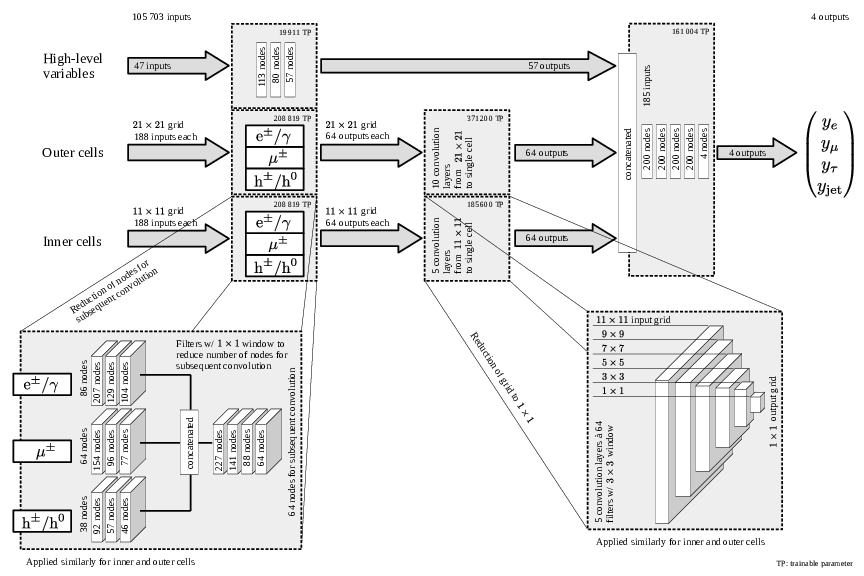
\includegraphics[width=\textwidth]{Figures/deeptau.png}
\caption{}
\label{fig:4tau_ccc}
\end{figure}